\documentclass{article}
\usepackage[T1]{fontenc}
\usepackage[utf8]{inputenc}
\usepackage[polish]{babel}
\usepackage{hyperref}
\usepackage{amsmath} 
\usepackage{float}
\usepackage{graphicx}
\usepackage{siunitx}




\title{Dokumentacja projektu: Inteligentna donica}
\author{
  Julia Dobroszek 251504 \\
  Aleksander Kaźmierczak 251544 (kierownik grupy)\\
  Malwina Wodnicka 251XXX \\  % Tutaj należy wstawić właściwy numer indeksu
}


\date{\today}

\begin{document}

\maketitle

%tabela opisujaca kto co robi
|%zrobic ladniejsza
\begin{table}[H]
    \centering
    \begin{tabular}{|c|c|}
    \hline
    członek zespołu & funkcjonalność\\
    \hline
    Olek & i2c, light, pwm, adc\\
    Malwina & gpio, audio, timer\\
    Julka & SPI, oled, czujnik temperatury\\
    \hline
    \end{tabular}
    \caption{Zawartość zespołu}
\end{table}


\section{Instrukcja użytkowania}

\subsection{Uruchomienie urządzenia}
Aby uruchomić inteligentną donicę, należy wykonać następujące kroki:
\begin{enumerate}
    \item Podłączyć urządzenie do źródła zasilania za pomocą dołączonego przewodu.
    \item Umieścić czujnik wilgotności (dwa metalowe druty) w glebie w doniczce. Czujnik powinien być umieszczony na głębokości około 3-5 cm, aby zapewnić prawidłowy pomiar wilgotności gleby.
    \item Po podłączeniu zasilania, system automatycznie rozpocznie pracę i wyświetli informacje na ekranie OLED.
    
\end{enumerate}


\subsection{Interpretacja wskaźników}
Inteligentna donica dostarcza użytkownikowi informacji o stanie rośliny poprzez:
\begin{enumerate} 
     \item \textbf{Wyświetlacz OLED} - Na ekranie prezentowane są aktualne statystyki dotyczące: 
     \begin{itemize} 
         \item Poziomu wilgotności gleby:
             \begin{itemize}
                \label{sec:wykorzystanie_ADC}
                 \item \textbf{sucho} - oznacza niski poziom wilgotności gleby (odczyt powyżej 2801), wskazujący na konieczność podlania rośliny
                 \item \textbf{w normie} - oznacza optymalny poziom wilgotności gleby (odczyt między 1601 a 2800), idealny dla wzrostu większości roślin
                 \item \textbf{mokro} - oznacza wysoki poziom wilgotności gleby (odczyt poniżej 1600), wskazujący na nadmiar wody, który może być szkodliwy dla rośliny
             \end{itemize}
         \item Temperatury otoczenia (w stopniach Celsjusza) 
         \item Natężenia światła - system interpretuje odczyt z czujnika i wyświetla jeden z trzech komunikatów:
         \begin{itemize}
             \item "jasno" - gdy wartość odczytu przekracza 2000
             \item "OK" - gdy wartość odczytu mieści się w przedziale od 350 do 2000
             \item "ciemno" - gdy wartość odczytu jest mniejsza niż 350
         \end{itemize}
         \item Dodatkowych informacji o stanie systemu 
     \end{itemize} 
     
     \item \textbf{Dioda RGB} - W zależności od poziomu wilgotności gleby, dioda RGB świeci się różnymi kolorami: 
     \begin{itemize} 
         \item Kolor żółto-zielony (\#c8ff1e) - oznacza stan \textbf{sucho} (odczyt powyżej 2801), sygnalizując potrzebę podlania rośliny
         \item Kolor zielony (\#1eff00) - oznacza stan \textbf{w normie} (odczyt między 1601 a 2800), sygnalizując optymalny poziom wilgotności
         \item Kolor błękitny (\#1effff) - oznacza stan \textbf{mokro} (odczyt poniżej 1600), sygnalizując nadmiar wody w glebie
     \end{itemize} 
 \end{enumerate}

\subsection{Kalibracja i konserwacja}
\begin{enumerate}
    \item \textbf{Kalibracja} - System został skalibrowany fabrycznie na podstawie eksperymentów empirycznych. Urządzenie nie posiada możliwości zewnętrznej kalibracji przez użytkownika.
    
    \item \textbf{Konserwacja} - Aby zapewnić prawidłowe działanie urządzenia:
    \begin{itemize}
        \item Regularnie czyścić czujnik wilgotności z osadów mineralnych, które mogą gromadzić się na jego powierzchni
        \item Utrzymywać wyświetlacz OLED w czystości, unikając bezpośredniego kontaktu z wodą
        \item Sprawdzać okresowo stan połączeń elektrycznych
        \item \textbf{Kategorycznie unikać kontaktu elektroniki z wodą} - Jedynym elementem, który może mieć bezpośredni kontakt z wilgocią, jest czujnik wilgotności (metalowe druty). Pozostałe elementy elektroniczne należy chronić przed zalaniem, zachlapaniem oraz nadmierną wilgotnością powietrza, gdyż może to prowadzić do trwałego uszkodzenia urządzenia i utraty gwarancji
    \end{itemize}
\end{enumerate}

\section{Funkcjonalności}

%olek
\subsection{Magistrala I2C}
\begin{enumerate}
    \item Interfejs I2C jest używany do komunikacji z czujnikiem światła oraz innymi komponentami wymagającymi komunikacji szeregowej. Implementacja obejmuje inicjalizację magistrali I2C, konfigurację adresów urządzeń oraz obsługę błędów komunikacji.
    \item Płytka LPC1769 posiada trzy magistrale I2C, w projekcie została użyta magistrala I2C2. 
    \item Czujnik światła jest podłączony do magistrali I2C2, a jego adres jest ustawiony na 0x44. Szczegóły konfiguracji znajdują się w sekcji \ref{sec:czujnik_swiatla}.
\end{enumerate}

\subsubsection{Omówienie rejestrów}
Rejestry mikroprocesora zostały opisane w tabeli 384. I2C register map w dokumentacji płytki. Poniżej znajdują się opisane rejestry:
\begin{itemize}
    \item \textbf{I2CONSET} - Rejestr ustawień kontrolnych I2C. Używany do ustawiania bitów w rejestrze kontrolnym I2CON. Pozwala ustawiać pojedyncze bity bez konieczności odczytywania i modyfikowania całego rejestru. Zapisanie '1' do bitu w tym rejestrze ustawia odpowiadający bit w rejestrze kontrolnym I2C. Poniżej zostały opiasne flagi:
    \begin{enumerate}
        \item Bity 0, 1 oraz 7:31 są zarezerowane 
        \item \textbf{AA} - Bit 2 \\
            Gdy:\\
            AA = 1 urządzenie wyśle ACK (czyli ustawi linię SDA w stan niski w czasie impulsu zegarowego na linii SCL). \\
            AA = 0 urządzenie wyśle NACK (czyli pozostawi linię SDA w stanie wysokim).
        \item \textbf{SI} - Bit 3 \\
            Flaga ta informuje o zmianie stanu magistrali np. zakończenie nadawania danych.
            Gdy:\\
            SI = 1, niski poziom sygnału SCL jest wydłużony. Transmisja zostaje wstrzymana.\\
            SI resetuje się poprzez zapisanie 1 do bitu SIC (SI Clear) w rejestrze I2CONCLR
        \item \textbf{STO} - Bit 4\\
            Flaga zakończenia transmisji danych. Jej działanie zależy od trybu, w jakim pracuje układ: master czy slave.\\
            W trybie master, ustawienie STO = 1 powoduje wysłanie warunku STOP na magistrali I2C, czyli SDA przechodzi z LOW na HIGH, gdy SCL jest HIGH. To kończy bieżącą transmisję i linia jest zwalniana.\\
            Gdy magistrala wykryje warunek STOP, flaga STO zostaje automatycznie wyczyszczona przez sprzęt.

        \item \textbf{STA} - Bit 5\\
            Służy do rozpoczęcia transmisji przez wysłanie warunku START
                \begin{itemize}
                    \item Jeżeli interfejs I2C jest w trybie slave, to:
                    \begin{itemize}
                        \item Interfejs przechodzi do trybu master
                        \item Jeśli magistrala jest wolna – natychmiast wysyła warunek START (SDA z HIGH do LOW przy SCL = HIGH).
                        \item Jeśli magistrala jest zajęta – czeka na warunek STOP, który „uwolni” magistralę, a potem wysyła START po pół okresie zegara wewnętrznego.
                    \end{itemize}

                    \item Jeśli interfejs już jest w trybie master, to:
                    \begin{itemize}
                        \item Ustawienie STA = 1 powoduje wysłanie repeated START – kolejnego warunku START bez wcześniejszego STOP.
                    \end{itemize}   
                    \item W przypadku, gdy STA oraz STO ustawimy jednocześnie na 1, to:
                    \begin{itemize}
                        \item w tybie master zostanie syłany sygnal STOP, następnie wysyłany jest START (restart transmisji)
                        \item w trybie slave nastąpi zatrzymanie transmisji bez wysłąnia STOP na magistralę, a następnie, jeśli magistrala jest wolna, zostanie wysłany START
                    \end{itemize}
                \end{itemize}
        \item \textbf{I2EN} - Bit 6\\
        Flaga odpowiedzialna za włączenie lub wyłączenie interfejsu I2C. Gdy:\\\
            I2EN = 0, interfejs I2C jest wyłączony\\
            I2EN = 1, interfejs I2C jest włączony
            
        
    \end{enumerate}
    \item \textbf{I2CONCLR} - Rejestr kasowania ustawień kontrolnych. Używany do kasowania bitów w rejestrze kontrolnym I2C. Zapisanie '1' do bitu w tym rejestrze kasuje odpowiadający bit w rejestrze kontrolnym I2C.
    \begin{enumerate}
        \item Bity 0, 1, 4 oraz 7:31 są zarezerowane
        \item \textbf{AAC} - Bit 2 - służy do wyzerowania bitu AA (Assert Acknowledge) w rejestrze I2CON. Bit AA odpowiada za to, czy urządzenie I2C nada ACK (potwierdzenie) podczas komunikacji.
        \item \textbf{SIC} - Bit 3 - służy do czyszczenia flagi przerwania I2C (Interrupt Clear). 
        \item \textbf{STAC} - Bit 5 - służy do czyszczenia flagi START (STA)
        \item \textbf{I2CENC} - Bit 6 - wyłącza interfejs I2C
    \end{enumerate}
    
    \item \textbf{I2STAT} - Rejestr statusu I2C. Dostarcza szczegółowe kody statusu pokazujące aktualny stan interfejsu. Z tego rejestru można tylko odczytywać dane.
    \begin{enumerate}
        \item Bity 0:2 oraz 8:31 są zarezerowane
        \item Bity 7:3 - zawierają kod aktualnego stanu interfejsu I2C.
            Kod statusu możemy wyodrębnić dzięki masce 0xF8:\\
            \begin{verbatim}
                uint8_t status = I2STAT & 0xF8;
            \end{verbatim}

            %dodac referencje do dokuemntacji lcp
            W rejestrze może wystąpić 26 kodów statusu. Kody, które mogą wystąpić znajdują się w dokumentacji LPC1769, w tabelach 399 oraz 402.\\
            Jeśli jakikolwiek z powyższych kodów wystąpi, to oznacza, że na pewno bit SI zostanie ustawiony na 1.
    \end{enumerate}
    
    
    \item \textbf{I2DAT} - Rejestr danych. Podczas trybu nadawania lub odbioru, dane (8 bitów) są zapisywane lub odczytywane z tego rejestru.   
    
    
    
    \item \textbf{I2SCLH} - Rejestr cyklu zegara SCL (wysoka połowa).Zawiera wysoką połowę cyklu zegara I2C.
    \item \textbf{I2SCLL} - Rejestr cyklu zegara SCL (niska połowa). Zawiera niską połowę cyklu zegara I2C.
    \item \textbf{MMCTRL} - Rejestr kontrolny trybu monitorowania. Używany do kontrolowania trybu monitorowania I2C.
    \item \textbf{I2DATA\_BUFFER} - Rejestr bufora danych I2C (Adres: 0x2C). Zawiera zawartość 8 najstarszych bitów rejestru przesuwnego I2DAT.
    
    \item \textbf{I2ADR0, I2ADR1, I2ADR2, I2ADR3} - Rejestry adresowe I2C. Zawierają 7-bitowy adres slave do działania interfejsu I2C w trybie slave. W na bicie 0 można ustawić czy urządzenie ma odpowiadać na GC (General Call) lub tylko na określony adres.
    \item \textbf{I2MASK0, I2MASK1, I2MASK2, I2MASK3} - Rejestry maski I2C. Służą do określenia dopasowania adresu w trybie slave.
\end{itemize}

\subsubsection{Inicjalizacja magistrali I2C2}
Inicjalizacja magistrali I2C2 odbywa się poprzez wykonanie następujących kroków:
\begin{enumerate}
    %opis ustawien konkretnych rejestrow w projekcie, uzasadnienie czemu wybralismy takie ustawienia
    \item Ustawienie odpowiednich pinów\\
        Użyte zostały piny P0.10 i P0.11, które odpowiadają pinom SCL i SDA na magistrali I2C2.\\
        Dla powyższych pinów wybrane zostały funkcje nr. 2, ponieważ z dokumentacji LPC1769 wynika, że funkcja nr. 2 odpowiada pinom SCL i SDA.\\ %odwolanie do tabeli w dokumentacji
    \item Włączenie zasilania magistrali I2C2\\
        % tabela Table 46. 
        Z tabeli 46. w dokumentacji LPC1769 można odczytać, że bit 6 w rejestrze PCONP odpowiada za włączenie zasilania magistrali I2C2.
        \[
            PCONP |= (1<<26)
        \]
    \item Ustawienie taktowania zegara\\
        Taktowanie zegara dla magistrali I2C2 ustawiamy poprzez wpisanie do rejestru I2SCLH i I2SCLL odpowiednich wartości. Wpierw pobieramy zawartość rejestru PCLK; robimy to poprzez odczytanie danych z bitów 21:20 z adresu 0x400F C1AC przy użyciu maski. Stąd wiemy, że dzielnikiem zegara jest 2, więc 
        \begin{align*}
        PCLK_{I2C2} &= \frac{CCLK}{2}\\
        I2SCLH &= \frac{PCLK_{I2C2}}{2 \cdot target\_clock}\\
        I2SCLL &= \frac{PCLK_{I2C2}}{target\_clock} - I2SCLH
        \end{align*}
            

        CCLK wynosi 100MHz. Mając powyższe wartości możemy wyliczyć taktowanie z poniższego wzoru:
        \[
        I2C_{bitfrequency} = \frac{PCLK}{I2SCLH + I2SCLL}
        \]
        Z Tabeli 395 w dokumentacji LPC1769 można odczytać, że standardowe taktowanie wynosi 100kHz, więc do rejestrów I2SCLH oraz I2SCLL wpisujemy 250
    \item Wyzerowanie flag rejestru I2CON\\
        W celu resetowania flag AC, STA, I2EN ustawiamy w rejestrze I2CONCLR bity 2, 5,6, które zerują te flagi w rejestrze I2CON.
        
    \item Włączenie magistrali I2C\\
        W celu włączenia magistrali I2C ustawiamy bit 6 w rejestrze I2CON.
\end{enumerate}

\subsubsection{Wykorzystanie magistrali I2C2}
\begin{enumerate}
    \item Początkowe ustawienia\\
        Rozpoczęcie transmisji odbywa się poprzez ustawienie flagi START w rejestraze I2CON (bit 5) na 1 oraz flagi SI (przerwanie) w rejestrze I2CON (5 bit) na 0. Później master czeka na zmianę flagi SI na 1, która oznacza, że transmisja została rozpoczęta. Następnie sprawdzany jest rejest stanu I2STAT, aby sprawdzić, czy warunek START został wysłany (0x08). Ustawiamy SI na 0.
    \item Wysyłanie danych\\
    \begin{enumerate}
        \item Wysyłanie adresu urządzenia. Adres urządzenia jest 7-bitowy. W rejestrze I2DAT należy wpisać adres urządzenia, a następnie ustawić pierwszy bit na 0, aby wskazać, że wysyłamy adres. Następnie ustawiamy flagę SI w rejestrze I2CON na 0.
        \item Master oczekuje na potwierdzenie (ACK) od slave - (z Tabeli 400) w rejestrze I2STAT powinna znajdowaćsię wartość 0x18. Gdy znajduje się tam inna wartość, to adres jest ponownie wysyłany.
        \item Po otrzymaniu ACK, master ustawia bit 5 w rejestrze I2CON (STA) na 0.
        \item Następnie master wysyła dane. W rejestrze I2DAT należy wpisać dane, które chcemy wysłać. Następnie ustawiamy flagę SI w rejestrze I2CON na 0.
        \item Oczekiwanie na ustawienie SI rejestru I2CON na 1
        \item Master oczekuje na potwierdzenie (ACK) od slave w rejestrze I2STAT powinna znajdowaćsię wartość 0x28. Gdy otrzymano ACK, to przechodzi do wysłania kolejnych danych.
    \end{enumerate}
    
    \item Odbieranie danych\\
    \begin{enumerate}
        \item Żeby wskazać adres urządzenia z któego będziemy odbierać dane należy wpisać 7-bitowy adres slave do rejestru I2DAT. Ponadto należy ustawić pierwszy bit na 1, aby wskazać, że odbieramy dane. Następnie ustawiamy flagę SI w rejestrze I2CON na 0.
        \item Master oczekuje na potwierdzenei (ACK) od slave - (z Tabeli 400) w rejestrze I2STAT powinna znajdowaćsię wartość 0x40. Gdy znajduje się tam inna wartość, to adres jest ponownie wysyłany.
        \item Po otrzymaniu ACK, master ustawia bit 5 w rejestrze I2CON (STA) na 0.
        \item Master ustawia bit 2 w rejestrze I2CON (AA) na 1, aby ustawić ACK. I odbiera bajty danych:
        \begin{enumerate}
            \item W rejestrze I2CON ustawiamy bit 3 (SI) na 0.
            \item Master czeka na zmianę flagi SI w rejestrze I2STAT
            \item Odczyt danych z I2DAT (8 bitów)
            \item przed ostatnim bajtem danych master ustawia bit 2 w rejestrze I2CON (AA) na 0, aby wyłączyć ACK.
        \end{enumerate}    
    \end{enumerate}    

    \label{sec:I2C_wysylanie_rejestrow}
    \item Zmiana i odczyt rejestrów urządzeń slave\\
    \begin{enumerate}
        \item Wysyłamy adres rejestru, który chcemy odczytać lub zmodyfikować.
        \item Jeśli chcemy modyfikować rejestr, należy wysłać nową wartość rejewstru.
        \item Jeśli chcemy odczytać, należy zacząć odbierać dane
        
    \end{enumerate}

    \item Koniec transmisji\\
    \begin{enumerate}
        \item W celu zakończenia transmisji należy ustawić bit 4 (STO) w rejestrze I2CON na 1.
        \item Zmiana wartości flagi SI w rejestrze I2CON na 0.
    \end{enumerate}


\end{enumerate}

%olek
\subsection{Czujnik światła}
\label{sec:czujnik_swiatla}
Inteligentna donica wykorzystuje czujnik światła oparty na protokole komunikacyjnym I2C. Implementacja tego elementu obejmuje trzy kluczowe funkcjonalności:
ISL29003 to zintegrowany czujnik światła z 16-bitowym przetwornikiem ADC. Wewnętrzny przetwornik ADC zapewnia 16-bitową rozdzielczość, jednocześnie odrzucając migotanie 50 Hz i 60 Hz spowodowane sztucznymi źródłami światła. Ogólne zasady działania ADC zostały przedstawione w rozdziale \ref{sec:ADC}.
%Malwina
\subsection{Sterowanie GPIO}
System wykorzystuje piny GPIO mikrokontrolera do sterowania różnymi elementami wykonawczymi donicy. Funkcjonalność ta obejmuje konfigurację kierunku pinów (wejście/wyjście), ustawianie stanów logicznych oraz obsługę przerwań sprzętowych. GPIO jest wykorzystywane między innymi do sterowania diodami sygnalizacyjnymi, wykrywania poziomu wody oraz obsługi przycisków interfejsu użytkownika.

\begin{enumerate}
    \item \textbf{Inicjalizacja i konfiguracja czujnika ISL29003} - Proces inicjalizacji obejmuje ustawienie adresu urządzenia na magistrali I2C, konfigurację rejestrów czujnika oraz określenie parametrów pomiaru, takich jak czułość i częstotliwość próbkowania.

    \item \textbf{Odczyt danych z czujnika} - Funkcjonalność ta odpowiada za komunikację z czujnikiem poprzez protokół I2C, wysyłanie komend odczytu do odpowiednich rejestrów oraz interpretację otrzymanych danych. Implementacja uwzględnia obsługę błędów komunikacji oraz weryfikację poprawności odczytanych wartości.

    \item \textbf{Przetwarzanie i analiza danych} - Po odczytaniu surowych danych z czujnika, system przetwarza je na użyteczne informacje o poziomie natężenia światła. Funkcjonalność ta obejmuje kalibrację, filtrowanie zakłóceń oraz konwersję wartości na jednostki zrozumiałe dla użytkownika (np. luxy).
\end{enumerate}

\subsubsection{Inicjalizacja czujnika ISL29003}
    Aby zainicjować czujnik ISL29003, należy ustawić wartość 1 na 7. bicie rejestru Command (0x00). Sposób wysyłania zawartości rejestró do urządzeń podrzędnych zostałopisany w poprzednim podrozdziale \ref{sec:I2C_wysylanie_rejestrow}.

    Wysyłanie adresu urządzenia - Wysyłanie adresu urządzenia ISL29003 na magistrali I2C. Adres urządzenia to 0x44.
    Informacje na temat rejestrów i ich wartości znajdują się w dokumentacji ISL29003, w tabeli 1.\\%odwolanie do dokumentacji

    Kolejnym etapem przygotowania czujnika do pracy jest zdefiniowanie zakresu. Stałe te będą używane do przeliczania danych wyjściowych czujnika. W naszym programie ustawiamy zakres na 3892, co oznacza skalę od 0 do 3892 lux. Aby ustawić wybrane przez nas wartości zakresu (range) należy sutawić bity 3:2 (tabela 9.) w rejestrze Control (0x01) na 0:1
%tabela 9.
    \begin{table}[H]
        \centering
        \begin{tabular}{|c|c|c|}
        \hline
        Bits 3:2 & k & RANGE (k)\\
        \hline
        0:0 & 1 & 973\\
        0:1 & 2 & 3892\\
        1:0 & 3 & 15,568\\
        1:1 & 4 & 62,272\\
        \hline
        \end{tabular}
        \caption{Zakresy skali lux}
    \end{table}
    Ustawiamy także liczbę cykli zegara na konwersację analogowo cyfrową poprzez umieszczenie wartości 0:0 na bitach 1:0 w rejestrze Command (0x00) (tabela 7.)
    \begin{table}[H]
        \centering
        \begin{tabular}{|c|c|}
        \hline
        BITS 1:0 & NUMBER OF CLOCK CYCLES\\
        \hline
        0:0 & $2^{16} = 65,536$\\
        0:1 & $2^{12} = 4,096$\\
        1:0 & $2^{8} = 256$\\
        1:1 & $2^{4} = 16$\\
        \hline
        \end{tabular}
        \caption{Liczby cykli zegara}
    \end{table}

    \subsubsection{Odczyt danych z czujnika}
    Dane z ISL29003 odczytujemy przy pomocy protokołu I2C. Dane wyjściowe przechowywane są w dchów rejestrach, ponieważ odczyt jest liczbą 16-bitową. W rejestrze o adresie 0x04 znajduje się najniższy bajt danych, a w rejestrze 0x05 najwyższy bajt. Sposób odczytywania danych został opisany w podrozdziale \ref{sec:I2C_wysylanie_rejestrow}.

    \subsubsection{Przetwarzanie i analiza danych}
    Po odczytaniu danych z czujnika, system przetwarza je na użyteczne informacje o poziomie natężenia światła. Aby uzyskać wartość w luxach, należy zastosować poniższy wzór (ten wzór obowiązuje tylko gdy mamy zewnętrzny rezystor 100k$\Omega$):\\
    \[
    E = \frac{FSR \cdot DATA}{2^{n}}
    \]
    Gdzie:\\
    E - wartość w luxach\\
    FSR - zakres skali (FSR = 3892 lux)\\
    DATA - odczytana wartość z rejestru\\
    n - liczba bitów w rejestrze (16 bitów)\\

    %wstawienie zdjęcia
    \begin{figure}[H]
        \centering
        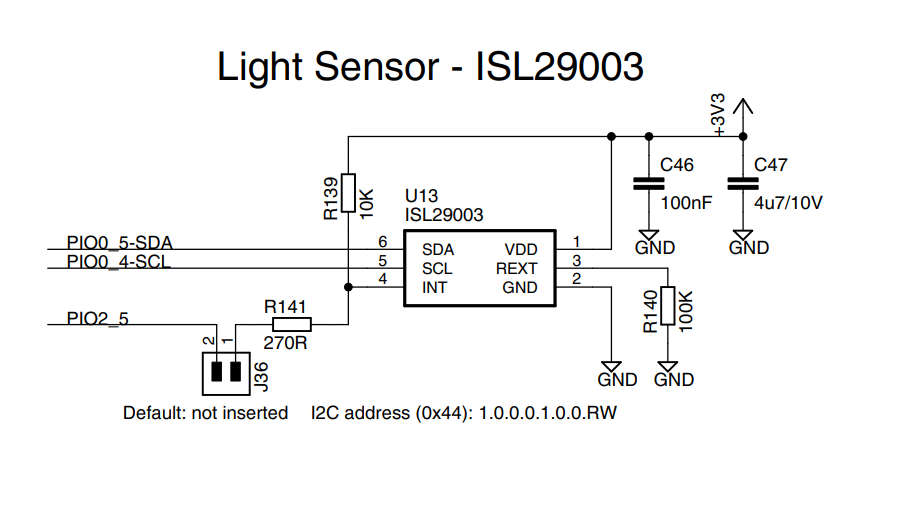
\includegraphics[width=0.8\textwidth]{doc/ISL29003/schemat.png}
        \caption{Schemat podłączenia czujnika ISL29003}
        \label{fig:czujnik_swiatla}
    \end{figure}





%Julka
\subsection{Czujnik temperatury}
System monitoruje temperaturę otoczenia rośliny za pomocą dedykowanego czujnika. Implementacja obejmuje:

\begin{enumerate}
    \item \textbf{Inicjalizacja czujnika temperatury} - Proces inicjalizacji obejmuje konfigurację czujnika z wykorzystaniem funkcji czasowych (getTicks) oraz ustawienie parametrów pomiaru.
    
    \item \textbf{Cykliczny odczyt temperatury} - Funkcjonalność ta odpowiada za regularne pobieranie danych z czujnika oraz konwersję odczytanych wartości na format zrozumiały dla użytkownika.
    
    \item \textbf{Wykorzystanie danych temperaturowych} - Informacja o temperaturze jest wyświetlana na ekranie OLED i może wpływać na decyzje systemu dotyczące nawadniania lub doświetlania rośliny.
\end{enumerate}

%Julka
\subsection{Magistrala SPI}
System wykorzystuje interfejs SPI do komunikacji z wyświetlaczem OLED oraz innymi peryferiami. Implementacja obejmuje konfigurację parametrów transmisji, takich jak częstotliwość zegara, tryb pracy oraz obsługę przerwań.

%Julka
\subsection{Wyświetlacz OLED}
Donica wykorzystuje wyświetlacz OLED model UG-9664HSWAG01 (oznaczenie na schemacie OLED1) komunikujący się przez interfejs SPI. Wyświetlacz bazuje na sterowniku SSD1305 132 x 64 Dot Matrix OLED/PLED Segment/Common Driver with Controller. Implementacja obejmuje inicjalizację wyświetlacza, konfigurację parametrów transmisji SPI oraz bibliotekę funkcji do wyświetlania informacji o stanie rośliny, poziomie światła i innych parametrach środowiskowych. Wyświetlacz służy jako interfejs użytkownika, prezentując dane w czytelnej formie graficznej.

%Malwina
\subsection{System audio}
System audio inteligentnej donicy składa się z głośnika (oznaczenie na schemacie SP1) oraz układu sterowania LM4811MM (oznaczenie na schemacie U10). Układ ten umożliwia generowanie sygnałów dźwiękowych informujących użytkownika o stanie rośliny. Implementacja obejmuje inicjalizację układu sterowania, konfigurację parametrów dźwięku oraz bibliotekę funkcji do odtwarzania różnych melodii w zależności od poziomu wilgotności gleby.


%Malwina
\subsection{Timer}
System wykorzystuje timery sprzętowe mikrokontrolera do precyzyjnego odmierzania czasu i wykonywania cyklicznych zadań. W przeciwieństwie do PWM, który służy do generowania sygnałów o zmiennym wypełnieniu, timery są wykorzystywane do wywoływania przerwań w określonych odstępach czasu. Funkcjonalność ta obejmuje konfigurację preskalerów, rejestrów porównania oraz obsługę przerwań. Timery są używane do planowania pomiarów, kontroli cykli nawadniania oraz implementacji funkcji oszczędzania energii.
%olek
\subsection{Modulacja szerokości impulsu (PWM)}
Implementacja PWM umożliwia precyzyjne sterowanie elementami wykonawczymi wymagającymi sygnału analogowego, takimi jak silniki czy regulacja jasności diody LED. Funkcjonalność obejmuje konfigurację częstotliwości sygnału PWM, ustawianie wypełnienia impulsu (duty cycle) oraz dynamiczną zmianę parametrów w zależności od warunków środowiskowych. PWM jest wykorzystywane do regulacji intensywności świecenia diod LED w diodzie RGB LED3 [schemat]. %dodaj schemat

\subsubsection{Inicjalizacja PWM}
\begin{enumerate}
    \item 
\end{enumerate}








%olek
\subsection{Przetwornik analogowo-cyfrowy (ADC)}
\label{sec:ADC}
System wykorzystuje przetwornik analogowo-cyfrowy do odczytu analogowego wejścia czujnika określanego jako "czujnik wilgotności". Należy zaznaczyć, że termin "wilgotność" jest w tym przypadku skrótem myślowym, ponieważ w rzeczywistości nie mierzymy bezpośrednio wilgotności gleby, a jej przewodność elektryczną, która jest skorelowana z zawartością wody w glebie. Implementacja obejmuje:
Wbudowany przetwornik ADC jest przetwornikiem 12-bitowym, co oznacza, że może zwracać wartość z zakresu 0-4095. Przetwornik ten działa przy użyciu metody SAR (Successive Approximation Register), która polega na sekwencyjnym przybliżaniu wartości.
\begin{enumerate}
    \item \textbf{Inicjalizacja i konfiguracja przetwornika ADC} - Proces inicjalizacji obejmuje konfigurację rejestrów mikrokontrolera, ustawienie częstotliwości próbkowania, wybór kanału pomiarowego oraz określenie napięcia referencyjnego. ADC może wykonać do 200 000 konwersji na sekundę (200 kHz), przy pełnej 12-bitowej rozdzielczości. To znaczy, że maksymalnie co 5 mikrosekund może być gotowy nowy wynik pomiaru. 
    
    \item \textbf{Odczyt wartości analogowej} - Funkcjonalność ta odpowiada za uruchomienie konwersji analogowo-cyfrowej, odczyt wyniku konwersji oraz obsługę ewentualnych błędów pomiaru.
    
    \item \textbf{Interpretacja danych pomiarowych} - System przetwarza odczytane wartości na względny poziom wilgotności gleby. Proces ten obejmuje kalibrację czujnika (określenie wartości dla suchej i mokrej gleby), filtrowanie zakłóceń oraz konwersję surowych danych na format zrozumiały dla użytkownika.
\end{enumerate}


%chapter 29.
\subsubsection{Inicjalizacja przetwornika ADC}
    \begin{enumerate}
        \item Na początku ustawiono piny do pracy w trybie analogowym. Dla pinu 23 na porcie 0 ustawiono funkcję nr. 1, co jest odpowiednikiem funkcji analogowej (Tabela 81.) \\%odwolanie do dokumentacji
              Aby ustawić wybraną funkcję, należy ustawić bity 15:14 w rejestrze PINSEL1 na 01.
        \item Następnie ustawiono 12. bit w rejestrze PCONP o adresie 0x400F C0C4 na 1, aby włączyć zasilanie dla przetwornika ADC.
        \item Kolejniym krokiem jest odczytanie dzielnika zapisanego w rejestrze PCLKSEL0 o adresie 0x400F C1A8 na bitach 25:24 (Tabela 40.). Domyślnie dzielnik ten wynosi 4 (w rejestrze pod podanymi bitami znajduje się 00). Wtedy obowiązuje wzór na PCLK:
        \[
        PCLK = \frac{CCLK}{4}
        \]
        Gdzie:\\
        CCLK - takt zegara układu; CCLK = 100MHz\\
        PCLK - takt zegara przetwornika ADC\\
        
    \end{enumerate}

\subsubsection{Obliczanie masek do odczytu wartości rejestrów}
        Aby móc zmieniać stan przetwarzania potrzebna jest maska, która pozwoli wybrać tylko interesujące nas bity z rejestru AD0CR.
        \begin{enumerate}
            \item W rejestrze AD0CR (0x4003 4000) na bicie 21 znajduje się informacja o stanie przetwornika:
            \begin{itemize}
                \item 0 - przetwornik jest gotowy do pracy;
                \item 1 - przetwornik jest wyłączony
            \end{itemize}
            \item Zatem potrzebujemy maski (1<<21)
        \end{enumerate}
\subsubsection{Ustawianie wartości AD0CR}
    W rejestrze AD0CR (0x4003 4000) na bitach 15:8 znajduje się wartość przez jaką dzielony jest PCLK, by uzyskać częstotliwość próbkowania.
    Zatem potrzebujemy maski \\
    \[
    (0xCLKDIV<<8) OR (1<<21)
    \]
    Gdzie:\\
    \begin{align*}
        \text{CLKDIV} = \text{rate} \cdot 65 \\
        \text{CLKDIV} = \frac{2 \cdot PCLK  + \text{CLKDIV}}{2 \cdot \text{CLKDIV}} - 1\\
    \end{align*}
    rate = 0,2MHz\\
    \\
    Aby ustawić wartość AD0CR, należy wykonać następujące kroki:
    \begin{enumerate}
        \item Wczytaj aktualną wartość rejestru AD0CR (0x4003 4000) do zmiennej.
        \item Wykonaj operację OR na tej zmiennej oraz masce.
        \item Zapisz zmienną z wynikiem do rejestru AD0CR
    \end{enumerate}
    W opisywanym projekcie przetwornik ADC nie korzysta z przerwań.

    \subsubsection{Przeliczanie odczytu na dane liczbowe}
    Jak napisano na początku podrozdziału, przetwornik ADC korzysta z metody SAR (Successive Approximation Register). SAR jest realizowany sprzętowo. Sposób działania przetwornika jest następujący:\\
    Dla uproszczenia przyjmujemy, że ADC ma 3 bity. Zakres wartości cyfrowych to 0-7. W rzeczywistości przetwornik ma 12 bitów.\\
    Zakładamy, że:

    \begin{align*}
        V_{\text{ref}} &= \SI{3.3}{\volt} \\
        V_{\text{in}} &= \SI{2.0}{\volt}
    \end{align*}
    Każdy krok, to 
    \begin{align*}
        \frac{\SI{3.3}{\volt}}{8} = \SI{0.4125}{\volt}
    \end{align*}

    \begin{enumerate}
        \item Ustawiamy najbardziej znaczący bit na 1, więc liczba wynoch 100.
        \item Następnie sprawdzamy, czy:
            \begin{align*}
                V_{\text{in}} \geq \frac{4}{8} \cdot V_{\text{ref}}\\
                \SI{2.0}{\volt} \geq \SI{1.65}{\volt}
            \end{align*}
        \item Tak, więc zachowujemy najstarszy bit i ustawiamy kolejny bit na 1, czyli 110.
        \item Następnie sprawdzamy, czy:
            \begin{align*}
                V_{\text{in}} \geq \frac{6}{8} \cdot V_{\text{ref}}\\
                \SI{2.0}{\volt} \geq \SI{2.475}{\volt}
            \end{align*}
        \item Nie, więc zmieniamy bit na 0, czyli 101. Ustawiamy kolejny bit na 1, czyli 101.
        \item Ponownie sprawdzamy, czy:
            \begin{align*}
                V_{\text{in}} \geq \frac{5}{8} \cdot V_{\text{ref}}\\
                \SI{2.0}{\volt} \geq \SI{2.06}{\volt}
            \end{align*}
        \item Nie, więc zmieniamy bit na 0, czyli 100. Wartość cyfrowa wynosi 100, czyli 4 w systemie dziesiętnym, co odpowiada lekko ponad połowie zakresu odczytu ($\frac{4}{7} \approx 0.57$, a stosunek $\frac{V_{\text{in}}}{V_{\text{ref}}} \approx 0.60$).
        
    \end{enumerate}
    Uzyskany pomiar służy do określenia wilgotności gleby i wypisanie na wyświtlacz odpowiedniego komunikatu, zostało to opisane w sekcji \ref{sec:wykorzystanie_ADC}.
%olek
\subsection{Komparator LM393}
Przeszukując sieć w poszukiwaniu dokumentacji komparatora LM393 nie mogliśmy znaleźć idealnie odpowiadającego opisu. Mimo, iż oznaczenia na układzie scalonym się pokrywają (dokumentacja dotyczy LM393), to wyprowadzenia nie są identyczne. W związku z tym nie udało się znaleźć dokładnego opisu, ale zasada działania przetwornika jest taka sama. 


\end{document}




